\documentclass{article}
\usepackage{multicol}
\usepackage{float}
\setlength{\columnsep}{1cm}

\usepackage{breakcites} % break citations so they don't spill over margin
% Center the section headers
\usepackage{sectsty}
% \usepackage{titlesec}
\usepackage{lipsum}
\sectionfont{\centering} % center just the titles

\usepackage[a4paper,right=18mm,left=18mm,top=25mm,bottom=25mm]{geometry} % https://www.sharelatex.com/blog/2013/08/06/thesis-series-pt2.html
\usepackage{pdfpages}

\usepackage[english]{babel}
\usepackage{inputenc}

 % insert clickable references and urls
\usepackage{url}
\usepackage{hyperref}
\graphicspath{ {images/final/} } % image path

\usepackage[nottoc]{tocbibind}

% Latex commands / macros
    \newcommand{\mat}[2][ccccccccccccccccccccccccccccccccccccccccccccc]
	    {\left[ \arraycolsep=4pt\def\arraystretch{1.5}
				\begin{array}{#1} #2 \\ 
				\end{array} 
		\right]}

	\newcommand{\crossmat}[1]{\mat{#1{^\times}}}

	\newcommand{\pvec}[1]{\vec{#1}\mkern2mu\vphantom{#1}}

    % Position vector macros
    \newcommand{\pspr}{\pvec{p}'_s} % position of the tool sphere (display)
    \newcommand{\ps}{\pvec{p}_s} % position of the tool rear (inertial)

    \newcommand{\prpr}{\pvec{p}'_r} % position of the tool rear (display)
    \newcommand{\pr}{\pvec{p}_r} % position of the tool rear (inertial)
    \newcommand{\pre}{\hat{\pvec{p}}_r}

    \newcommand{\pfpr}{\pvec{p}'_f}
    \newcommand{\pf}{\pvec{p}_f}
    \newcommand{\pfe}{\hat{\pvec{p}}_f}

    \newcommand{\pc}{\pvec{p}_c}
    \newcommand{\pd}{\pvec{p}_d}

    \newcommand{\pu}{\pvec{p}_u}

    % Attitude macros
    \newcommand{\A}{\mathbf{A}} % attitude of the display
    \newcommand{\Ad}{\mathbf{A}_d} % attitude of the display
    \newcommand{\Ac}{\mathbf{A}_c} % attitude of the camera
    \newcommand{\At}{\mathbf{A}_t} % attitude of the tool
    \newcommand{\Atpr}{\mathbf{A}'_t} % attitude of the tool

    \newcommand{\Adinv}{\mathbf{A}^{-1}_d} % attitude of the display
    \newcommand{\Acinv}{\mathbf{A}^{-1}_c} % attitude of the camera
    \newcommand{\Atinv}{\mathbf{A}^{-1}_t} % attitude of the tool

    % Quaternion macros
	\newcommand{\q}{\overline{\mathbf{q}}}
	\newcommand{\qc}{\q_c}
	\newcommand{\qd}{\q_d}
	\newcommand{\qt}{\q_t}

    % Error quaternions
	\newcommand{\dq}{\delta\q_t}
	\newcommand{\dqw}{\delta q_4}
    \newcommand{\dqvec}{\delta \vec{q}}

    \newcommand{\dt}{\delta\theta}
    \newcommand{\dtvec}{\delta\vec{\theta}}

	% Covariance matrix macros
    \newcommand{\cov}{\mathbf{\Sigma}}

    % Quaternion error covariances
	\newcommand{\Pqc}{\mathbf{\Sigma}_{qc}}
	\newcommand{\Pqd}{\mathbf{\Sigma}_{qd}}
	\newcommand{\Pqt}{\mathbf{\Sigma}_{qt}}

    % Angular error covariances
	\newcommand{\Ptc}{\mathbf{\Sigma}_{\theta c}}
	\newcommand{\Ptd}{\mathbf{\Sigma}_{\theta d}}
	\newcommand{\Ptt}{\mathbf{\Sigma}_{\theta t}}

	\newcommand{\Pacpr}{\mathbf{\Sigma}'_{ac}}
	\newcommand{\Padpr}{\mathbf{\Sigma}'_{ad}}
	\newcommand{\Patpr}{\mathbf{\Sigma}'_{at}}

	\newcommand{\Pps}{\mathbf{\Sigma}_{ps}}
	\newcommand{\Ppr}{\mathbf{\Sigma}_{pr}}
	\newcommand{\Ppf}{\mathbf{\Sigma}_{pf}}
	\newcommand{\Ppc}{\mathbf{\Sigma}_{pc}}
	\newcommand{\Ppd}{\mathbf{\Sigma}_{pd}}
    \newcommand{\Ppl}{\mathbf{\Sigma}_{l}}

	\newcommand{\Ppspr}{\mathbf{\Sigma}'_{ps}}
	\newcommand{\Pprpr}{\mathbf{\Sigma}'_{pr}}
	\newcommand{\Ppfpr}{\mathbf{\Sigma}'_{pf}}

	% Tool length macro
	\newcommand{\pl}{\vec{p}_l}
    \newcommand{\ple}{\hat{\vec{p}}_l}
    \newcommand{\plpr}{\pvec{p}'_l}

	% Section header commands
    \renewcommand{\thesection}{\Roman{section}.} 
    \renewcommand{\thesubsection}{\Alph{subsection}.}
    \renewcommand{\thesubsubsection}{\thesubsection\arabic{subsubsection}}

	% Miscelanous macros
	\newcommand{\tab}{ \textrm{ \ \ \ \ } }

    \newcommand{\z}{\mathbf{\vec{z}}}
    \newcommand{\y}{\mathbf{\vec{y}}}
    \newcommand{\x}{\mathbf{\vec{x}}}

    % Object tracking commands
    \newcommand{\xd}{\dot{x}}
    \newcommand{\xdd}{\ddot{x}}

    \newcommand{\deg}{^{\circ} }
    \newcommand{\Hz}{\textrm{Hz}}

    \newcommand{\deldq}{\frac{\partial \pl}{\partial \dqvec} }
    \newcommand{\ddq}{\frac{\partial}{\partial \dqvec} }



%%%%%%%%%%%%%%%%%%%%%%%%%%%%%%%%%%%%%%%%%%%%%%%%%%%%%%%%%%%%%%%%%%%%%%%%%%%%%%%
%% TITLE PAGE
%%%%%%%%%%%%%%%%%%%%%%%%%%%%%%%%%%%%%%%%%%%%%%%%%%%%%%%%%%%%%%%%%%%%%%%%%%%%%%%

\begin{document}
% https://en.wikibooks.org/wiki/LaTeX/Title_Creation
% \begin{titlepage}

	\title{The 3D Interaction Tool: A Pointing Device for Virtual Reality Applications}
	\author{Lukas Gemar}
	\date{March 26, 2016}
	\maketitle

% \end{titlepage}


%%%%%%%%%%%%%%%%%%%%%%%%%%%%%%%%%%%%%%%%%%%%%%%%%%%%%%%%%%%%%%%%%%%%%%%%%%%%%%%
%% Abstract
%%%%%%%%%%%%%%%%%%%%%%%%%%%%%%%%%%%%%%%%%%%%%%%%%%%%%%%%%%%%%%%%%%%%%%%%%%%%%%%

\begin{abstract}
The 3D Interaction Tool is a hand-held device that enables a user to interact with virtual reality applications. Since both the position and orientation of the tool are tracked, user input with the tool accomplishes tasks such as selecting, translating, and rotating three-dimensional objects, or free-hand drawing in space. The tool�s position is tracked by a software application that filters observations from a camera attached to the virtual reality display, and the orientation is found by means of observations from an inertial measurement unit attached to the tool itself. Simple computer-aided design and drawing applications demonstrate the capabilities of the 3D Interaction Tool. 
\end{abstract}

% \begin{multicols}{2}
\begin{flushleft}

\section{Nomenclature}

% Position vector definitions
\textbf{Position vectors definitions in the inertial coordinate frame}: \\
$ \ps \equiv $ position of the spherical tracking target on tool rear \\
$ \pr \equiv $ position of the tool rear \\
$ \pf \equiv $ position of the tool front \\
$ \pc \equiv $ position of the tracking camera \\
$ \pd \equiv $ position of the virtual reality display \\

\medskip

% Rotated position vector definitions
\textbf{Rotated position vectors}: \\
$ \pspr \equiv $ position of the spherical tracking target on tool rear, camera coordinates \\
$ \prpr \equiv $ position of the tool rear in display coordinates \\
$ \pfpr \equiv $ position of the tool front in display coordinates \\

\medskip

% Attitude matrix definitions
\textbf{Attitude matrices}: \\
$ \Ac \equiv $ attitude of the tracking camera \\
$ \Ad \equiv $ attitude of the virtual reality display \\
$ \At \equiv $ attitude of the interaction tool \\
$ \Atpr \equiv $ attitude of the interaction tool in display coordinates \\

\medskip

% Quaternion definitions
\textbf{Body-referenced quaternion representations of attitude}: \\
$ \qc \equiv $ attitude of the tracking camera \\
$ \qd \equiv $ attitude of the virtual reality display \\
$ \qt \equiv $ attitude of the interaction tool \\

\medskip

% Covariance definitions
\textbf{Position error covariances in inertial coordinate frame}: \\
$ \Pps \equiv $ covariance of spherical tracking target position \\
$ \Ppr \equiv $ covariance of the position of the rear of the interaction tool\\
$ \Ppf \equiv $ covariance of the position of the front of the interaction tool\\
$ \Ppc \equiv $ covariance of the position of the tracking camera \\
$ \Ppd \equiv $ covariance of the position of the virtual reality display \\

\medskip

\textbf{Attitude error covariances in the inertial coordinate frame}: \\
$ \Pqc \equiv $ covariance of the tracking camera attitude quaternion error \\
$ \Pqd \equiv $ covariance of the display attitude quaternion error \\
$ \Pqt \equiv $ covariance of the interaction tool attitude quaternion error \\

\medskip

\textbf{Position error covariances in rotated body coordinates}: \\
$ \Ppspr \equiv $ covariance of the sphereical tracking target position \\
$ \Pprpr \equiv $ covariance of the position of the rear of the interaction tool \\
$ \Ppfpr \equiv $ covariance of the position of the front of the interaction tool \\

\medskip

\textbf{Attitude error covariances in the rotated body coordinates}: \\
$ \Pacpr \equiv $ covariance of the tracking camera attitude angular error \\
$ \Padpr \equiv $ covariance of the display attitude angular error \\
$ \Patpr \equiv $ covariance of the interaction tool attitude angular error \\

%%%%%%%%%%%%%%%%%%%%%%%%%%%%%%%%%%%%%%%%%%%%%%%%%%%%%%%%%%%%%%%%%%%%%%%%%%%%%%%
%% INTRODUCTION
%%%%%%%%%%%%%%%%%%%%%%%%%%%%%%%%%%%%%%%%%%%%%%%%%%%%%%%%%%%%%%%%%%%%%%%%%%%%%%%

\section{Introduction}

\subsection{Motivation}

As much as \$25 billion could be spent on virtual reality (VR) and augmented reality (AR) software applications by 2025 \cite{Bloomberg-01-13}. There are two primary modes of user-input that are possible for these applications: indirect and direct. Indirect input devices translate the user's physical movements into the motion of a virtual cursor by means of a fixed transformation. Common examples of indirect input devices are a mouse or joystick. Direct input devices also translate physical to virtual movements, but this transformation is one-to-one. For example, a touch screen is a direct input device because the physical location of the user's press is colocated with the virtual click. 

\medskip

With the advent of virtual reality applications the following question must be answered: which of these input paradigms -- indirect or direct -- will prove most useful for interacting with virtual reality applications? While indirect input devices have achieved widespread popularity for two-dimensional displays, the direct input paradigm for VR applications embraces the immersiveness of VR experiences by enabling intuitive interactions for users. Direct input devices allow users to reach out and interact with the objects of their virtual space, just as they would with objects in their physical space. 


\subsection{Background}

\subsection{Usability Objectives}

The usability requirements presented in Figure \ref{fig:usability} must be met for the tool to succeed as an \textit{input} device for VR software applications.

\begin{figure}[H]
	\begin{center}
		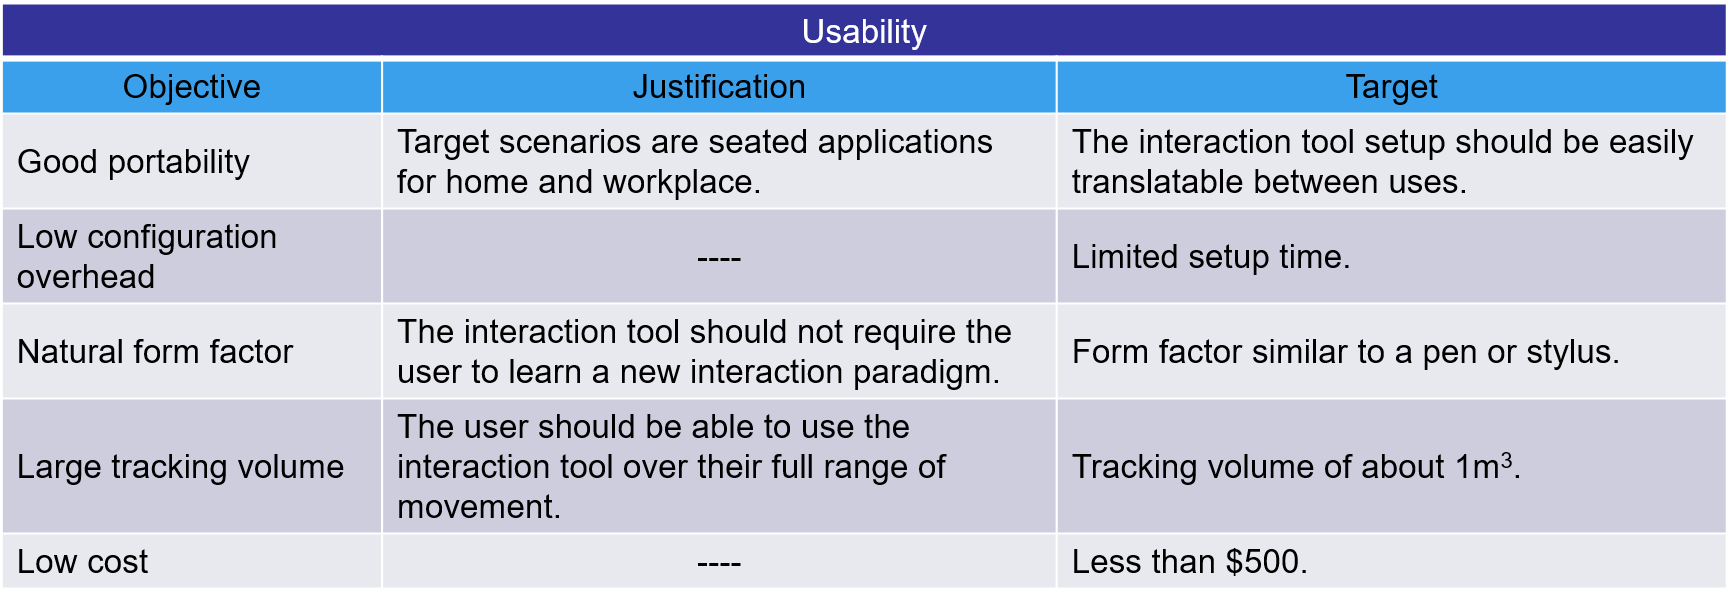
\includegraphics[width=0.5\textwidth]{Usability}
	\end{center}
	\caption{Usability design objectives}
	\label{fig:usability}
\end{figure}

\subsection{Performance Objectives}

The performance requirements presented in Figure \ref{fig:performance} must be met for the tool to succeed as a \textit{direct} input device for VR software applications.

\begin{figure}[H]
	\begin{center}
		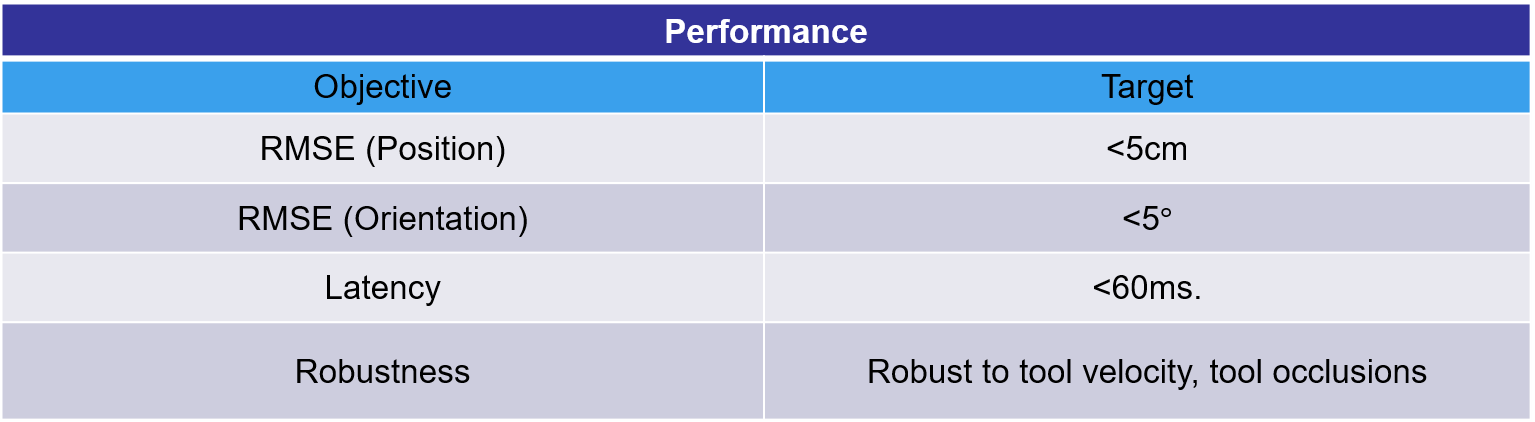
\includegraphics[width=0.5\textwidth]{Performance}
	\end{center}
	\caption{Performance design objectives}
	\label{fig:performance}
\end{figure}

%%%%%%%%%%%%%%%%%%%%%%%%%%%%%%%%%%%%%%%%%%%%%%%%%%%%%%%%%%%%%%%%%%%%%%%%%%%%%%%
%% Tracking system design
%%%%%%%%%%%%%%%%%%%%%%%%%%%%%%%%%%%%%%%%%%%%%%%%%%%%%%%%%%%%%%%%%%%%%%%%%%%%%%%

\section{Design}

\subsection{Requirements}

In order to enable direct input with the interaction tool, the tool's tracking system must estimate both the position and orientation of the interaction tool. Additionally, rendering a virtual representation of the tool requires measuring its position and orientation relative to the virtual reality display orientation, given by the attitude matrix $\Ad$. To track the tool's absolute trajectory, its position is determined relative to the world -- that is, relative to a non-accelerating, inertial coordinate system in the user's physical environment. The position and orientation of the tool in the world coordinates of the inertial frame are $\pf$ and $\At$, respectively. The position of the tool in the coordinate frame of the virtual reality display is denoted by a 'prime' sign: the tip or front of the tool in display coordinates is $\pfpr$. Thus, there are four tracking targets: $\pf$, $\At$, $\pfpr$, and $\Ad$; these are shown in Figure \ref{fig:requirements}. 

\begin{figure}[H]
	\begin{center}
		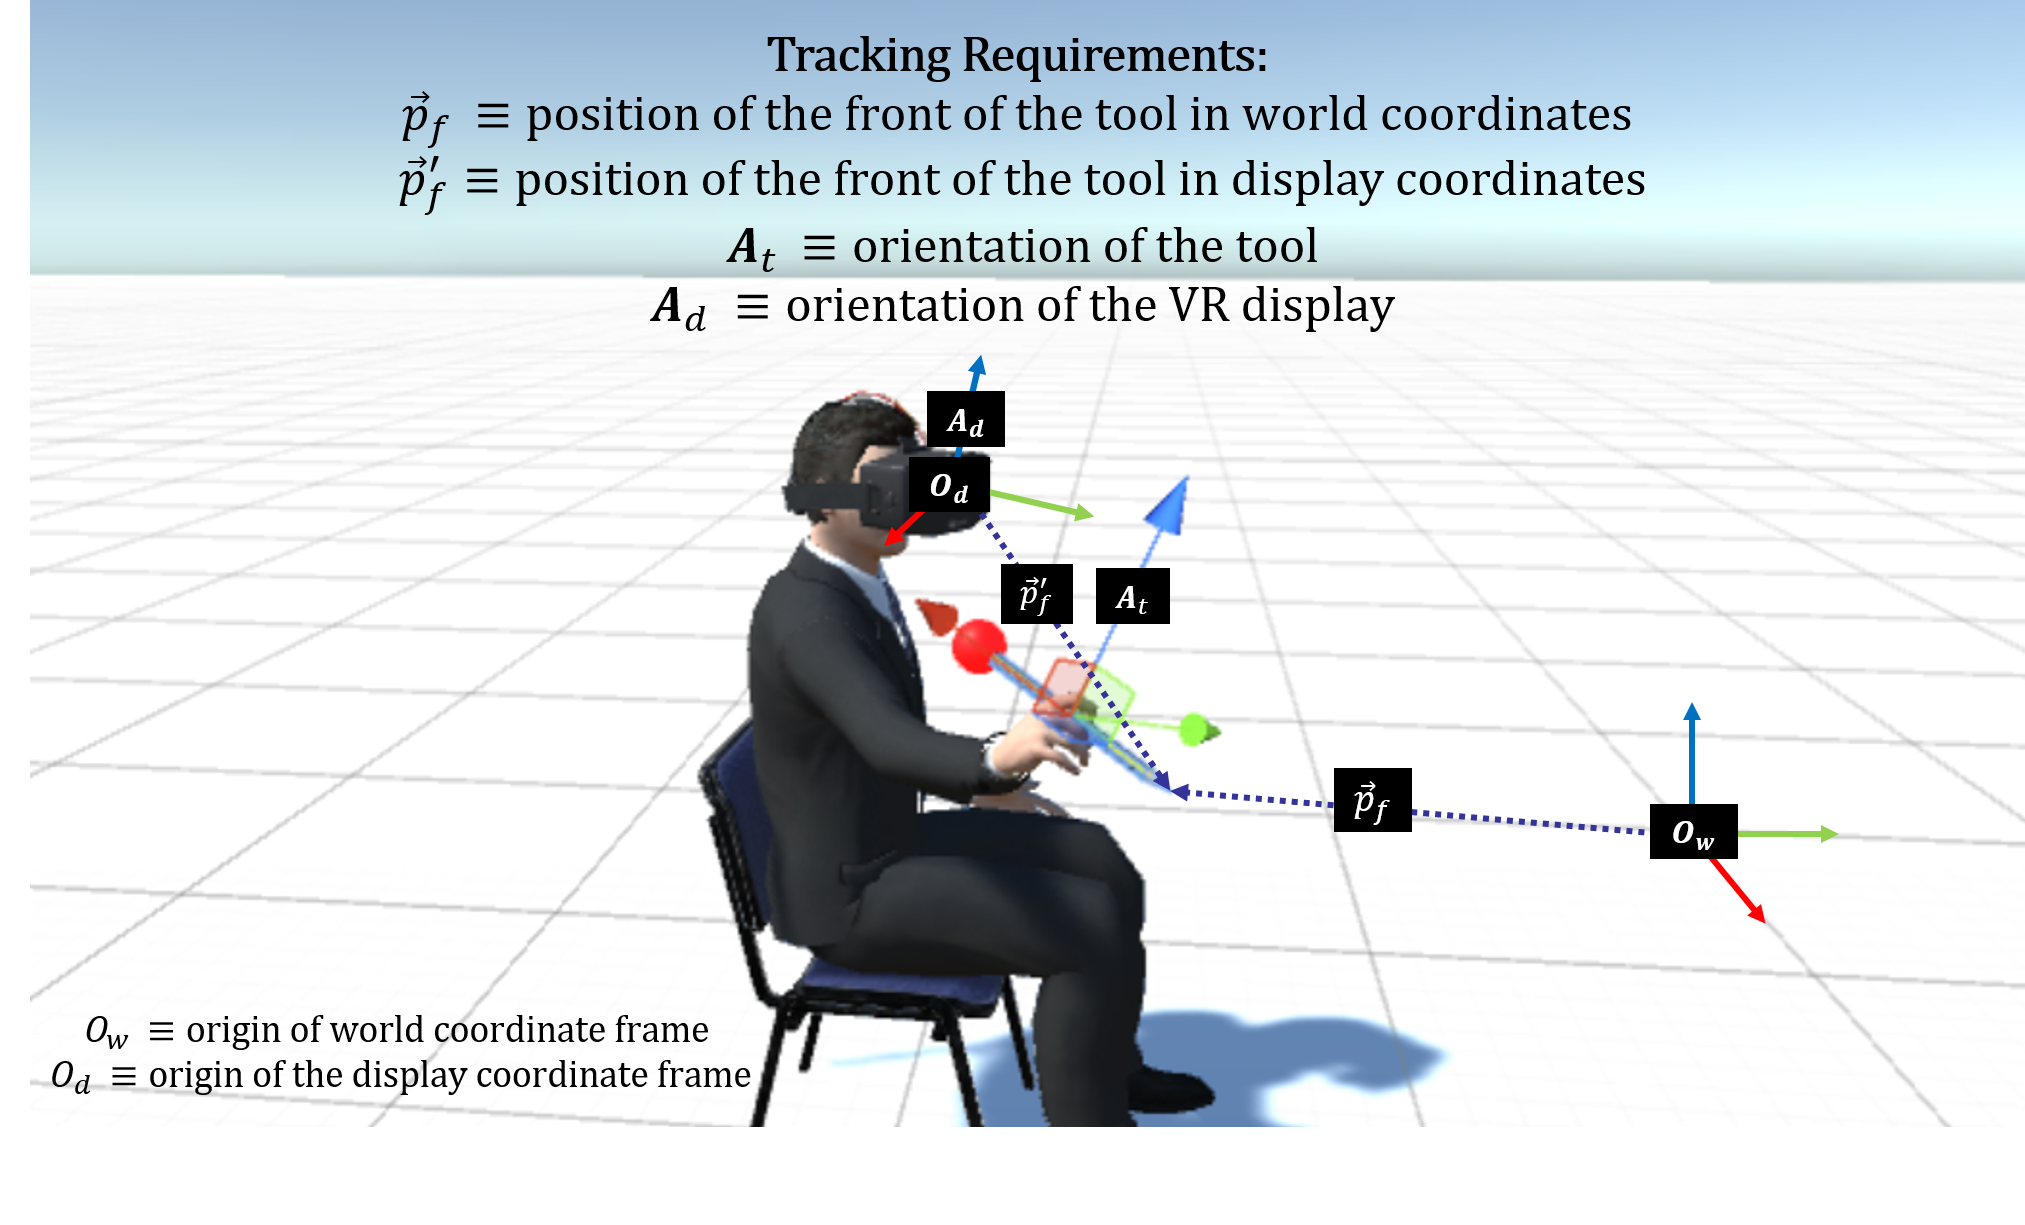
\includegraphics[width=0.5\textwidth]{requirements}
	\end{center}
	\caption{Position and orientation tracking requirements}
	\label{fig:requirements}
\end{figure}

\subsection{Geometry}

The geometry of the tool tracking system affects both the usability and the performance of the interaction tool. The display-referenced geometry is chosen because it eliminates the burden on the user to pre-calibrate their environment before providing direct input to VR applications. At the same time, this geometry is compatible with VR applications with which a user interacts while seated.

\subsubsection{Option 1: World-referenced geometry}

The world-referenced tracking geometry is shown in Figure \ref{fig:worldtopo}.

\begin{figure}[H]
	\begin{center}
		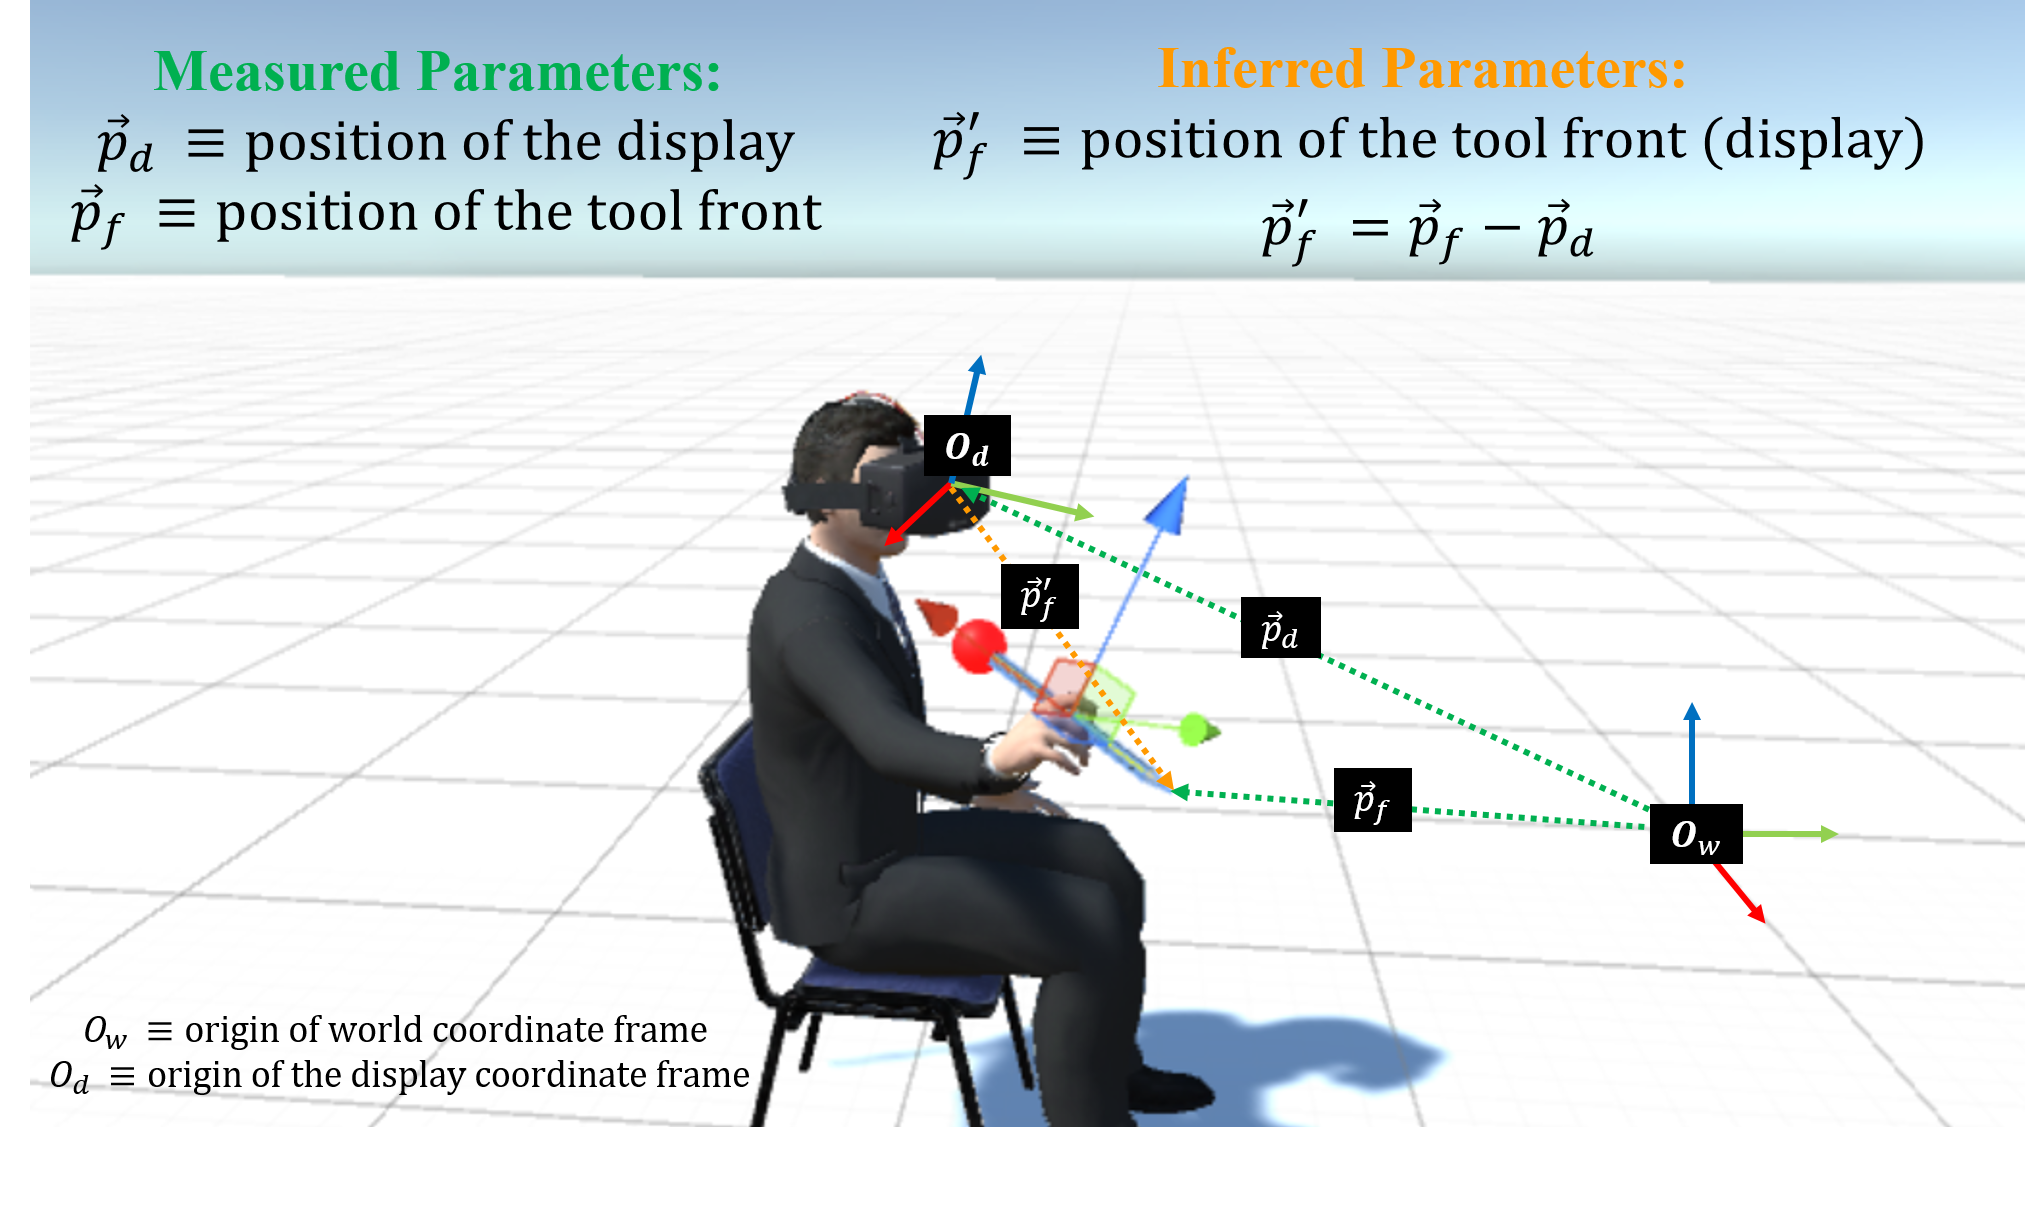
\includegraphics[width=0.5\textwidth]{WorldTopo}
	\end{center}
	\caption{Position tracking with a world-referenced geometry}
	\label{fig:worldtopo}
\end{figure}

\subsubsection{Option 2: Display-referenced geometry}

The display-referenced tracking geometry is shown in Figure \ref{fig:displaytopo}.

\begin{figure}[H]
	\begin{center}
		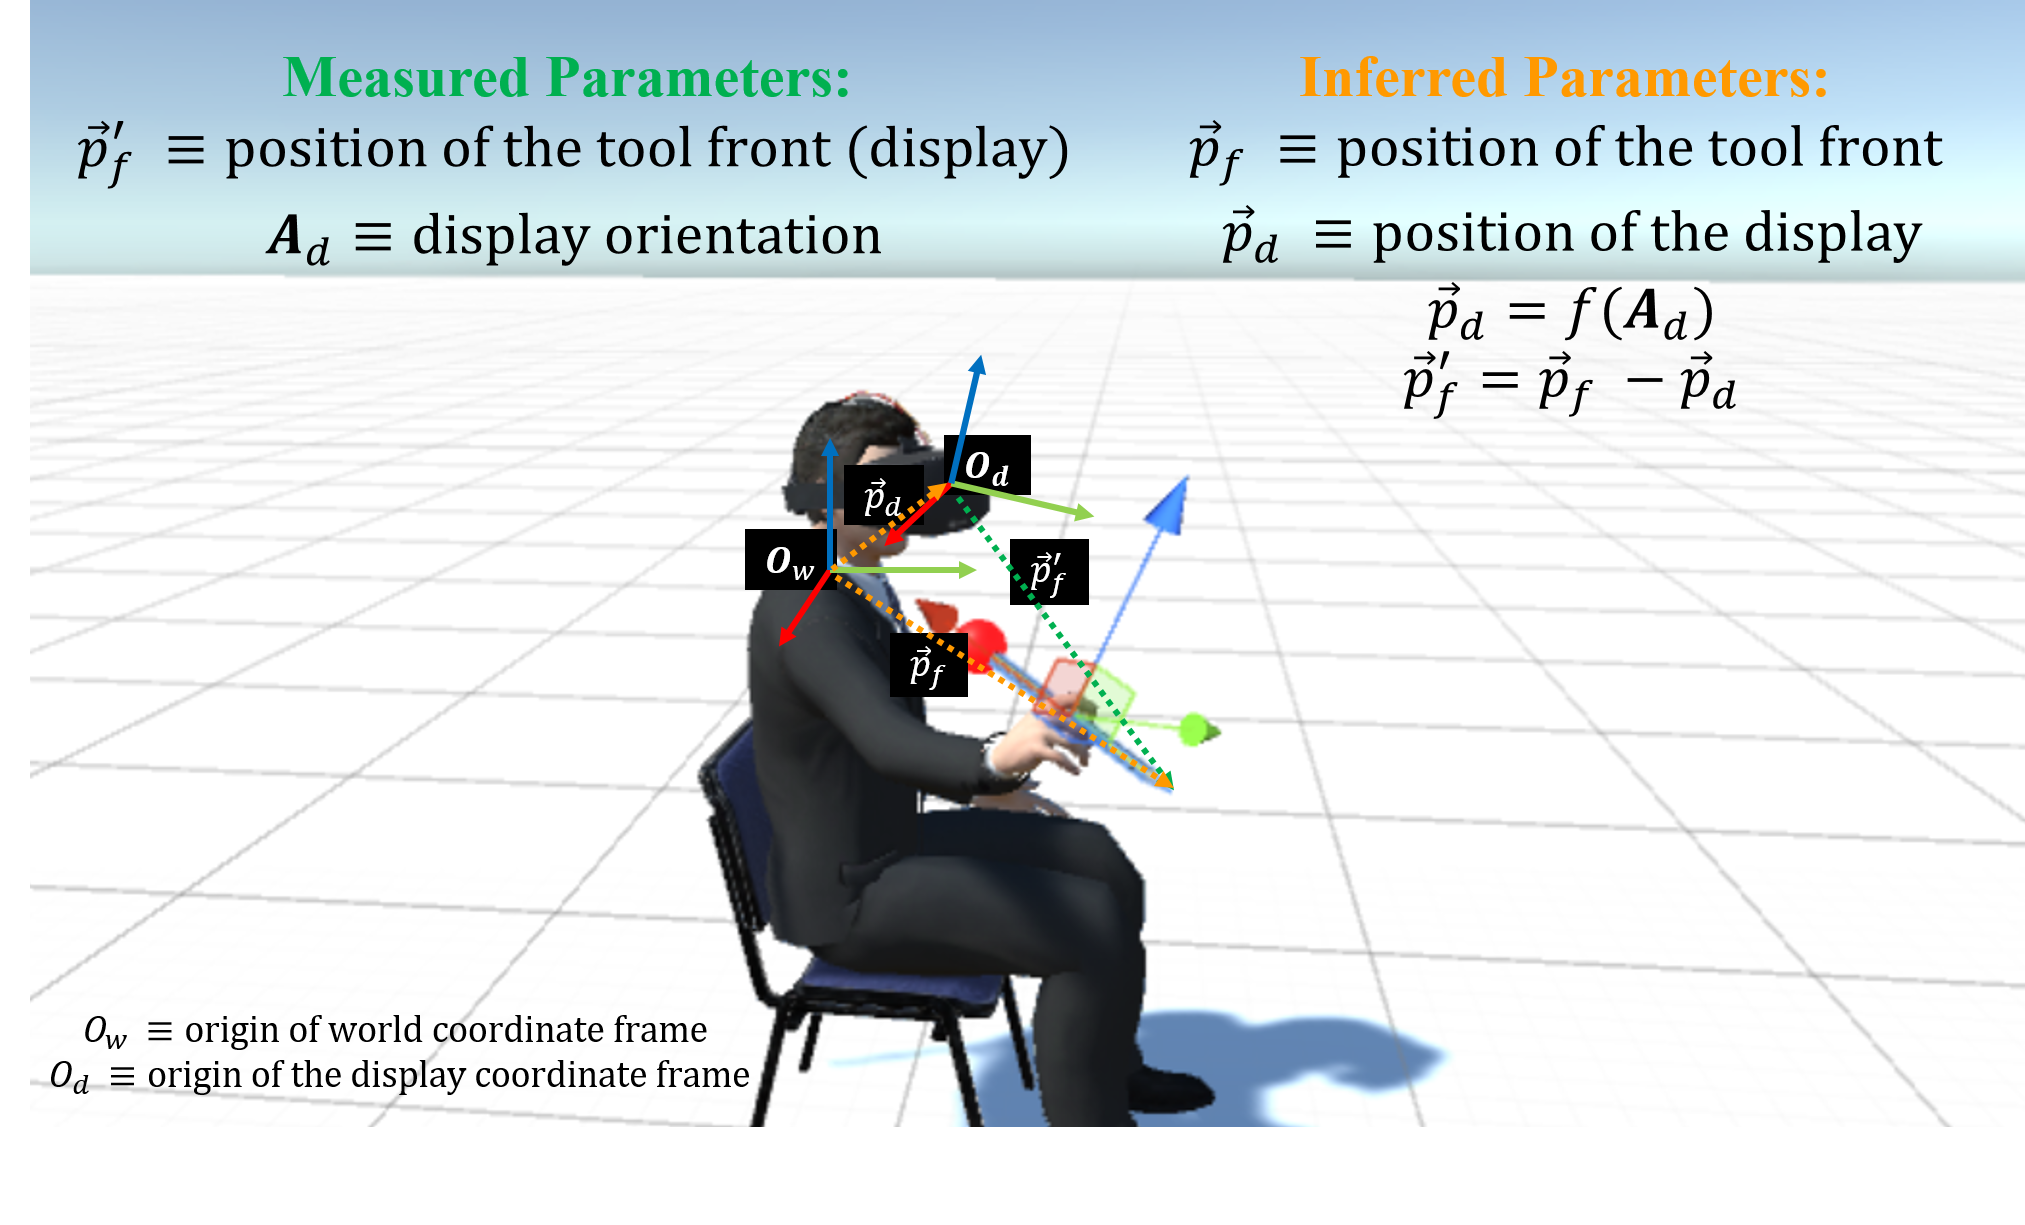
\includegraphics[width=0.5\textwidth]{DisplayTopo}
	\end{center}
	\caption{Position tracking with a display-referenced geometry}
	\label{fig:displaytopo}
\end{figure}

\subsubsection{Geometry Selection: Comparing portability and tracking volume}

Tracking geometries 1 and 2 have advantages and disadvantages when evaluated using the usability design objectives. Relative to the usability criteria, the two geometries differ greatly in their portability and tracking volume. 

\medskip

The world-referenced tracking geometry requires a fixed coordinate system in the user's physical environment, decreasing portability by increasing the configuration overhead for using the direct input device. However, once this coordinate system is established, the user can provide direct input to a VR application over a very large tracking volume, up to the size of the room in which the tracking system is located. The display-referenced geometry, on the other hand, has the advantage of enabling a user to provide direct input to a VR application without pre-calibrating the physical environment in which they are using the VR display. The tradoff is that the tracking volume is small. Since the origin of the world coordinate system in the display-referenced geometry is located beneath the user's head, the user must remain seated while using a direct input device with a display-referenced tracking geometry.

\subsection{Technology}

A combination between optical and inertial sensors was chosen to track the 3D Interaction Tool's position and orientation. The chart in Figure \ref{fig:trackingtech} summarizes the comparison between various alternatives for the choice of the tracking technology.

\begin{figure}[H]
	\begin{center}
		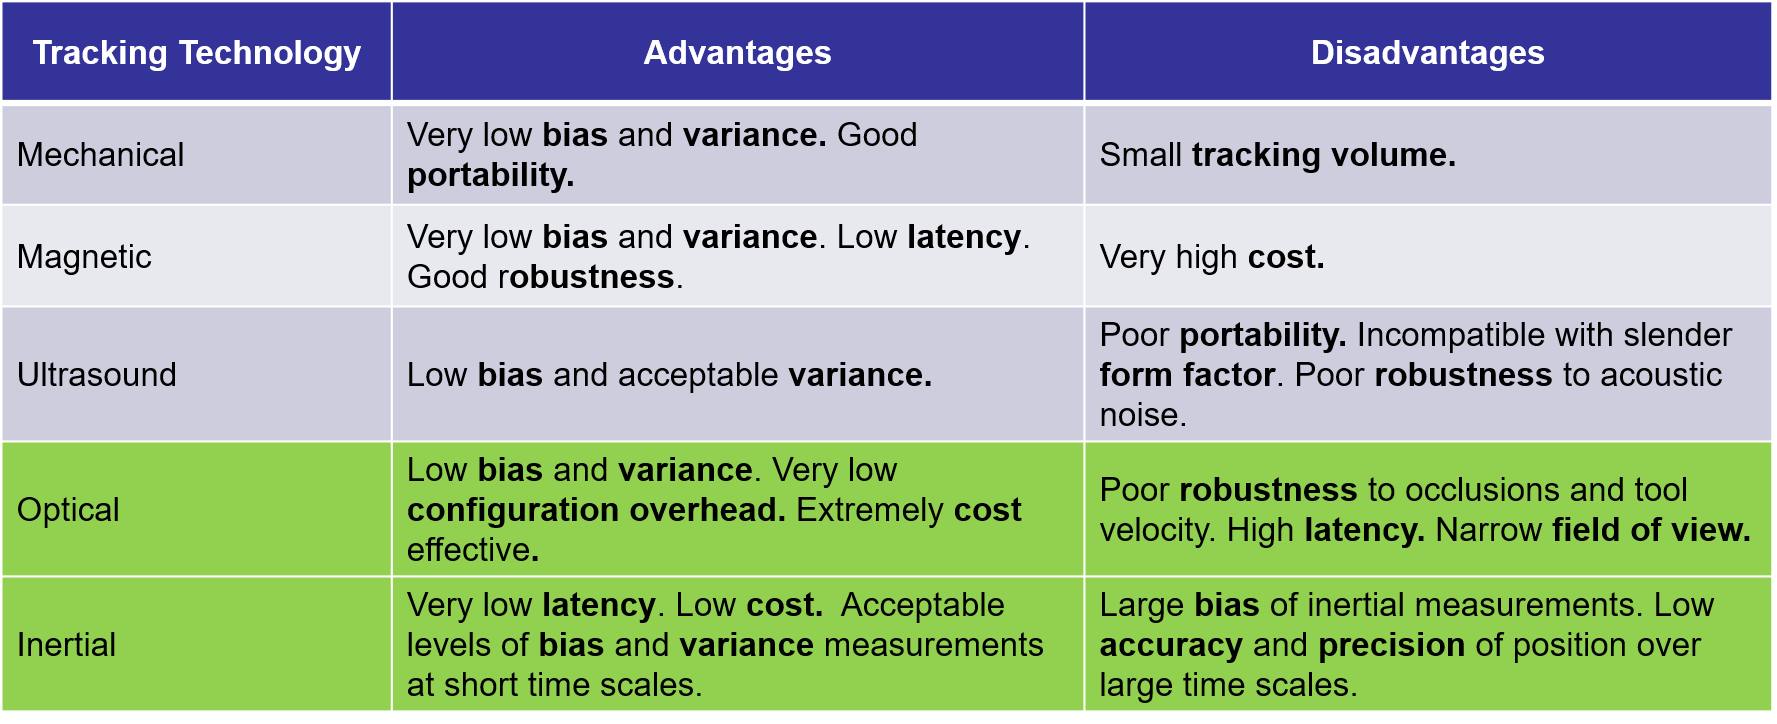
\includegraphics[width=0.5\textwidth]{TrackingTech}
	\end{center}
	\caption{Comparison of five tracking technologies}
	\label{fig:trackingtech}
\end{figure}

%%%%%%%%%%%%%%%%%%%%%%%%%%%%%%%%%%%%%%%%%%%%%%%%%%%%%%%%%%%%%%%%%%%%%%%%%%%%%%%
%% Final Design
\subsection{Final Design}

The final system layout is shown in figure \ref{fig:finaldesign}.

\begin{figure}[H]
	\begin{center}
		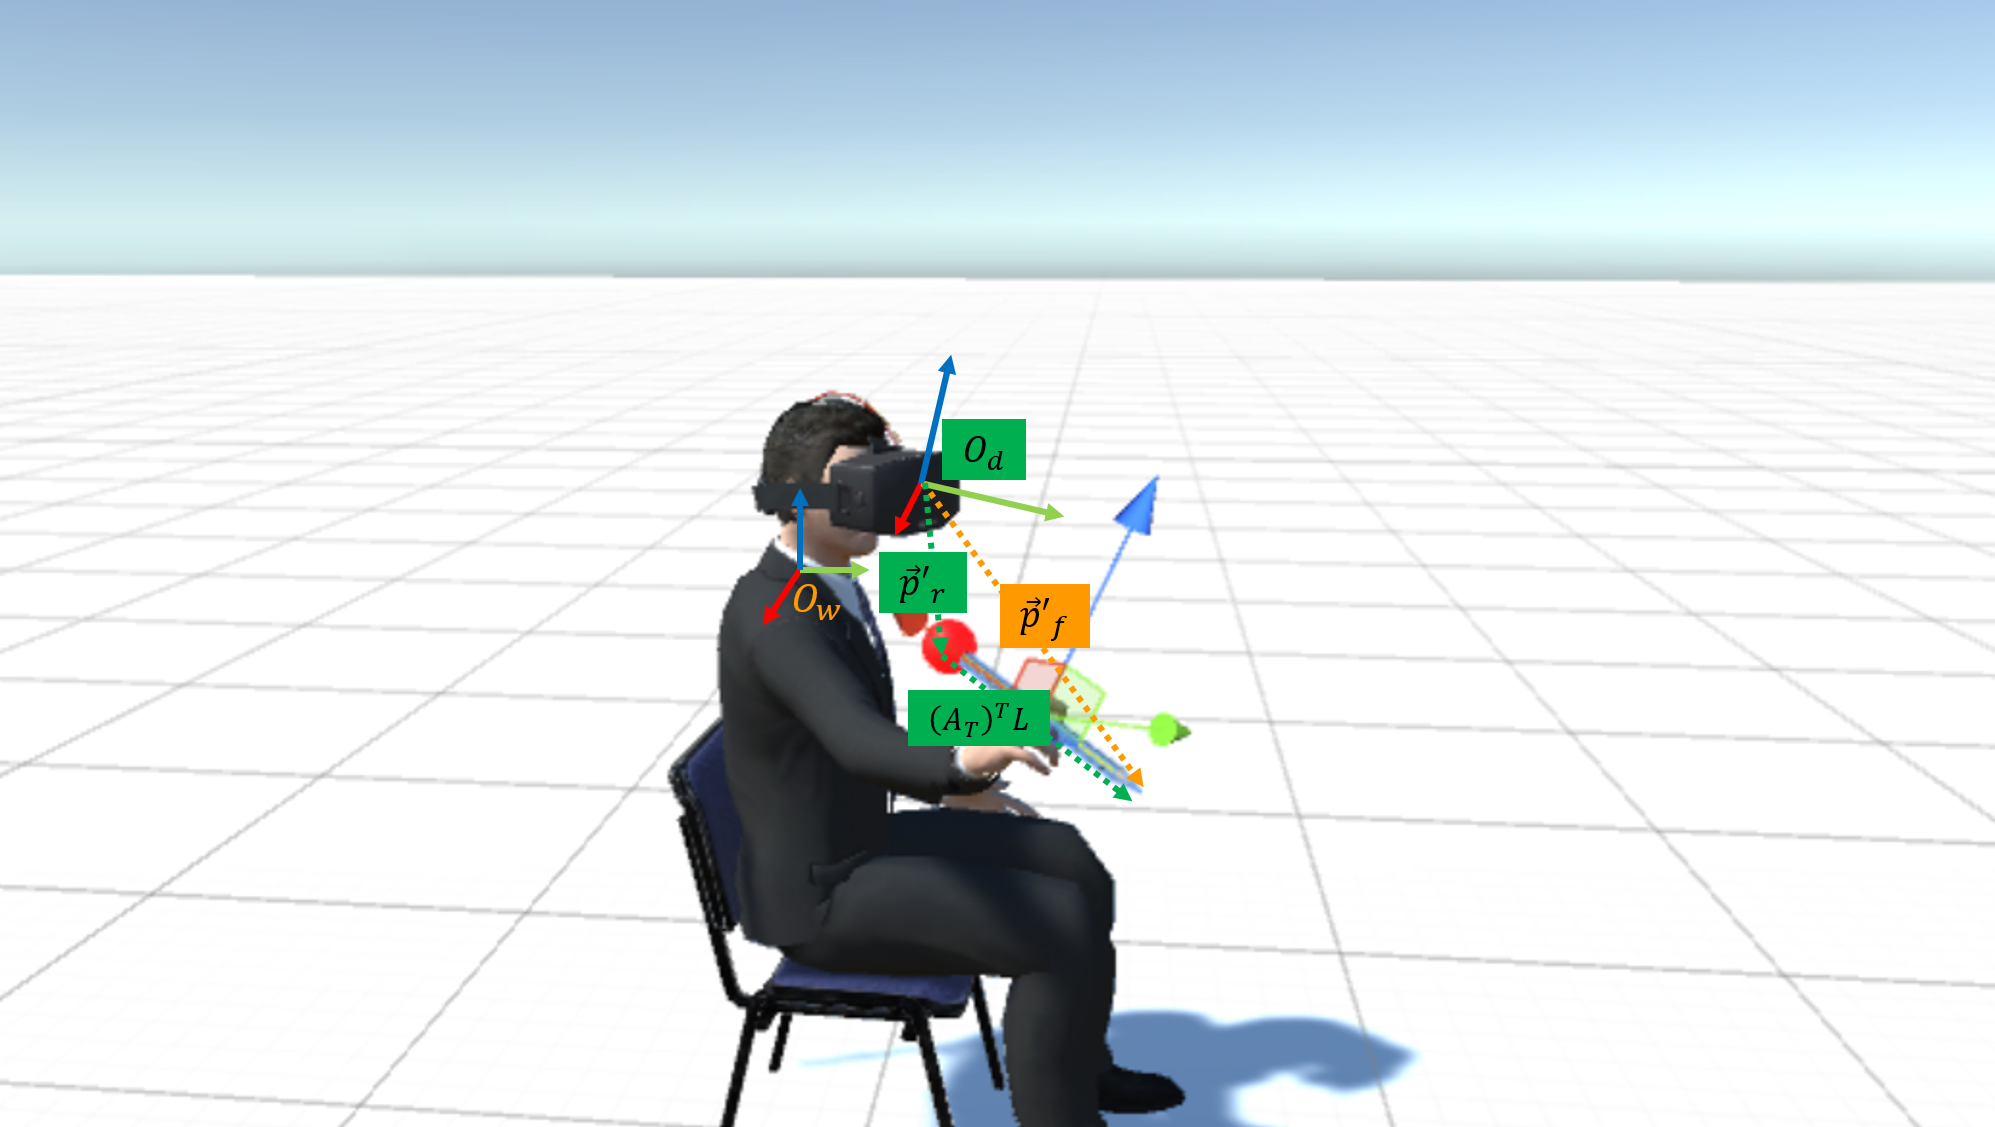
\includegraphics[width=0.5\textwidth]{FinalDesign}
	\end{center}
    \caption{Final tracking system design: a display-referenced tracking topology}
	\label{fig:finaldesign}
\end{figure}

%% Inferring the tool position
\subsubsection{Tracking measurements}

Not all of these three tracking targets are measured directly. The tracking targets are inferred from the measurements of the position of the rear of the interaction tool relative to the camera, the attitude of the camera, and the attitude of the tool. The position of the tool relative to the camera is denoted by $\pspr$, the attitude of the camera relative to the inertial coordinate system by $\Ac$ and the attitude of the tool relative to the inertial coordinate system by $\At$. The vector $\pspr$ is measured by finding the .

%% Inferring the tool position
\subsubsection{Inferring the tool position}

The position of the front of the tool in world coordinates is given by $\pf$. This position is inferred through measurements of the position of the rear of the tool and the tool's orientation. The equation for the position of the front of the tool is 

$$ \pf = \pr + \Atinv \pl $$

where the position of the rear of the tool, $\pr$ is given by

$$ \pr = \Acinv \pspr - \pc $$

The attitude matrix, $\Atinv$, is the rotation from the body coordinates of the tool to the world coordinate system.

In order to render the tool on the display for the user, the position of the tool must be known to the VR application in the coordinate system of the VR display. The position of the front of the tool in display coordinates is $\pfpr$ and it is found by multiplying the tool's position in the world coordinate system by the attitude of the display. Additionally, the position of the display must be added to the tool position before multiplying by the display attitude matrix:

$$ \pfpr = \Ad (\pf + \pd) $$

The tool attitude in the coordinate system of the display is denoted by $\Atpr$ and it is found by composing the rotation from the tool's body coordinates to world coordinates with the display attitude matrix: 

$$ \Atpr = \Ad \Atinv \pl $$

This is the tool orientation visible to the user. 

%%%%%%%%%%%%%%%%%%%%%%%%%%%%%%%%%%%%%%%%%%%%%%%%%%%%%%%%%%%%%%%%%%%%%%%%%%%%%%%
%% Implementation
%%%%%%%%%%%%%%%%%%%%%%%%%%%%%%%%%%%%%%%%%%%%%%%%%%%%%%%%%%%%%%%%%%%%%%%%%%%%%%%
\section{Implementation}

The system's physical layout is shown in \ref{fig:systemlayout}. For simplicity, the tracking camera is assumed to be fixed. The model for this system is geometrically equivalent to the one presented in Figure \ref{fig:finaldesign}. The webcam of the computer is used as the tracking camera. The inertial measurement unit, the Adafruit BNO055, is attached to the breadboard. A colored foam sphere is attached to the rear of the interaction tool to serve as the tracking target.

\begin{figure}[H]
	\begin{center}
		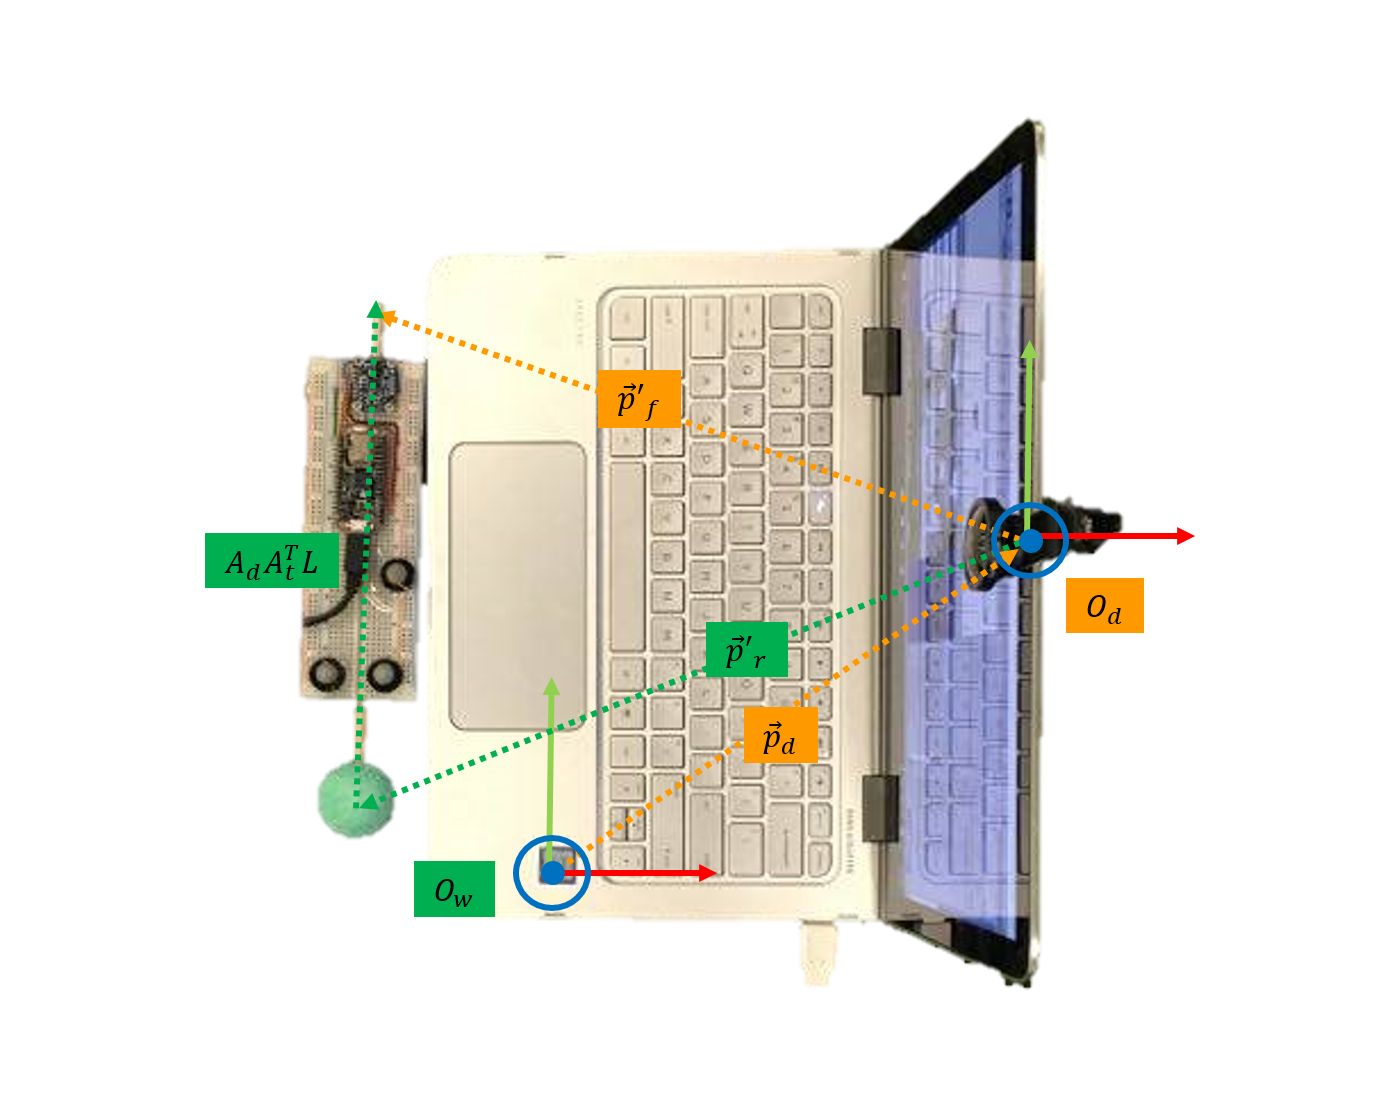
\includegraphics[width=0.5\textwidth]{SystemLayout}
	\end{center}
    \caption{Geometrically equivalent tracking system}
	\label{fig:systemdiagram}
\end{figure}

The virtual reality application runs on the computer shown in Figure \ref{fig:systemlayout}. While this virtual reality application is not immersive, it creates a virtual 3D environment displayed to the user on the computer screen, where they can interact with virtual objects. Thus, this geometry is sufficient to prove the usefulness of the 3D Interaction Tool for virtual reality applications.

The spherical tracking target is chosen because its size in each image does not depend on its orientation. Additionally, if the angle subtended by the tracking target in the field of view is small, then the midpoint of the tracking target in world coordinates is on the same plane as the vanishing points on the edges of the target.

The block diagram of the implmented tracking system is shown in Figure \ref{fig:systemdiagram}.

\begin{figure}[H]
	\begin{center}
		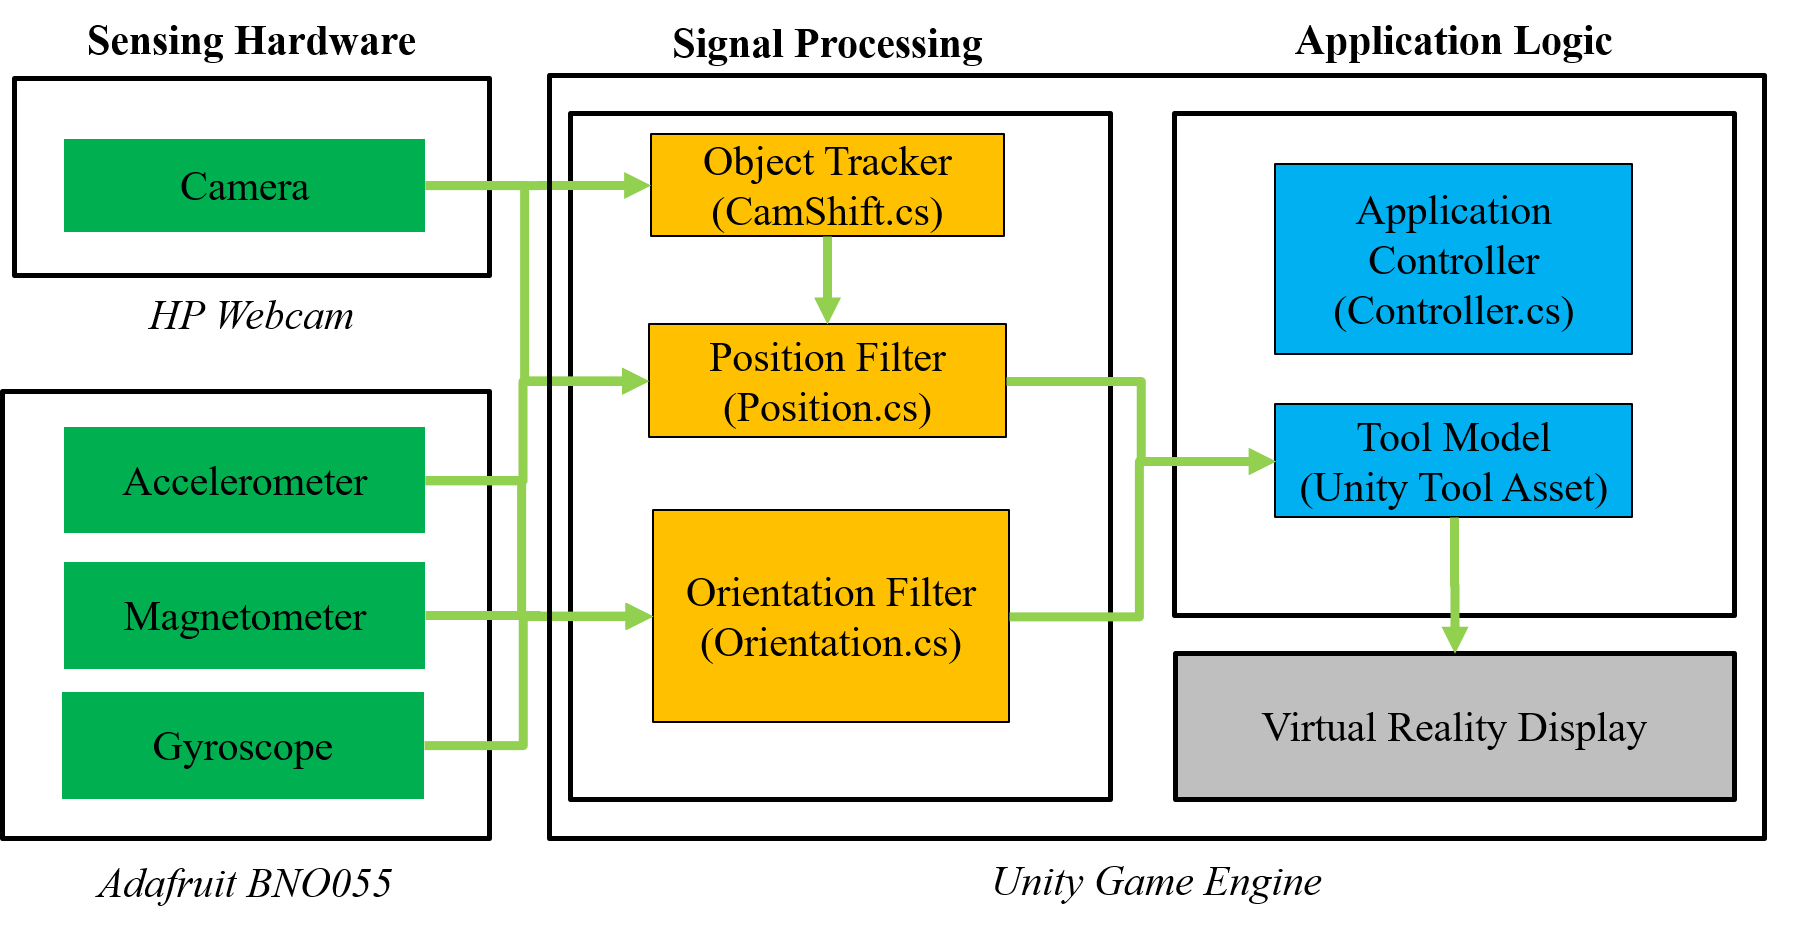
\includegraphics[width=0.5\textwidth]{SystemDiagram}
	\end{center}
    \caption{Full system diagram of implementation}
	\label{fig:systemdiagram}
\end{figure}


%%%%%%%%%%%%%%%%%%%%%%%%%%%%%%%%%%%%%%%%%%%%%%%%%%%%%%%%%%%%%%%%%%%%%%%%%%%%%%%
%% Orientation tracking
%%%%%%%%%%%%%%%%%%%%%%%%%%%%%%%%%%%%%%%%%%%%%%%%%%%%%%%%%%%%%%%%%%%%%%%%%%%%%%%
\section{Orientation Tracking}

\subsection{Mathematical Representation of Orientation}
The orientation of the interaction tool relative to the world coordinate frame can be represented in a number of ways. The two representations that will be important here are the attitude matrix and the attitude quaternion. First, the attitude of the orientation tool can be described by the attitude matrix $A$. The attitude matrix typically maps a vector in the reference frame to a vector in the the body frame \cite{Markley2007}. This mapping is given by the relation, 

\[ \bf{b} = A \bf{r} \]

Second, the attitude of the interaction tool can be represented as a quaternion. A rotation in three-dimensions is equivalent to an axis of rotation and and angle of rotation. If $\hat{n}$ is the axis of a rotation and $\theta$ is the angle of the rotation, then the quaternion $\overline{q}$ represents the attitude: 

\[ \overline{q} = \mat{\vec{q} \\ q_4} \] 

with $\vec{q} = \hat{n} \sin{\frac{\theta}{2}}$ and $q_4 = \cos{\frac{\theta}{2}}$. The quaternion must have length 1: $\overline{q}^T \overline{q} = 1$. 

The attitude matrix and the quaternion representing attitude are related by the following equation, where $A$ is a function of $\overline{q}$ \cite{Shuster1982}: 

\[ A(\overline{q}) = (q_4^2 - {\| \vec{q} \|}^2) I_{3x3} + 2 \vec{q}\vec{q}^T - 2 q_4 [\vec{q}\times] \]

where ${[\vec{q}\times}]$ is the skew-symmetric cross product matrix, 

\[ [\vec{q}\times] = \mat{ 0 & -q_3 & q_2 \\ q_3 & 0 & -q_1 \\ -q_2 & q_1 & 0} \]

The relationship between $A$ and $\overline{q}$ can also be expressed as the product of two matrices \cite{Markley2007}: 

\[ A(\overline{q}) = \Xi(\overline{q})^{T} \Psi(\overline{q}) \]

with 

\[ \Xi(\overline{q}) = \mat{q_4 \bf{I}_{3x3} + [\vec{q}\times] \\ -\vec{q}^T } \]

\[ \Psi(\overline{q}) = \mat{q_4 \bf{I}_{3x3} - [\vec{q}\times] \\ -\vec{q}^T } \]

\subsection{Naive Measurement Model}

The TRIAD estimation method finds the attitude matrix $A$ that maps three reference frame vectors $\vec{r}_k$ to their corresponding body frame vectors $\vec{b}_k$ for $k = 1, 2, 3$ \cite{Shuster2004}. Two observations of reference frame vectors provide sufficient information to compute a right-handed orthonormal triad of vectors in the reference frame. If $\vec{v}_1$ and $\vec{v}_2$ are reference frame vectors for the accelerometer and the magnetometer, respecitively, then 

$$ \vec{v}_1 = \mat{ 0 \\ 0 \\ 9.81 } \tab \textrm{and} \tab \vec{v}_2 = \mat{ 0.3 & \\ -1 & \\ 0 } $$ 

so that the gravity vector points down and the magnetometer vector points in the direction of magnetic North in Boston, relative to the world reference frame. The orthonormal vector triad representing the reference frame is given by, 

$$ 	\vec{r}_1 = \frac{\vec{v}_1}{\| \vec{v}_1 \|}, \tab \vec{r}_2 = \frac{\vec{v}_1 \times \vec{v}_2}{\| \vec{v}_1 \times \vec{v}_2 \|}, \tab \vec{r}_3 = \vec{r}_1 \times \vec{r}_2 $$

Let $\vec{w}_1$ be the measurement of the normalized unit vector from the accelerometer and $\vec{w}_2$ be the measurement of the normalized unit vector from the magnetometer, then the orthonormal vector triads for the reference vectors are given by, 

$$ \vec{b}_1 = \frac{\vec{w}_1}{\| \vec{w}_1 \|}, \tab \vec{b}_2 = \frac{\vec{w}_1 \times \vec{w}_2}{\| \vec{w}_1 \times \vec{w}_2 \|}, \tab \vec{b}_3 = \vec{w}_1 \times \vec{w}_2 $$

If there was no noise in the system, then it would be the case that $\vec{b}_k = A \vec{r}_k$ for $k=1,2,3$. An equivalent way of writing this in matrix form is the following: 

$$ M_b = A M_r $$ 

where 

$$ M_b = \mat{ \vec{b}_1 & \vec{b}_2 & \vec{b}_3 } $$
$$ M_r = \mat{ \vec{r}_1 & \vec{r}_2 & \vec{r}_3 } $$

Since $M_r$ is an orthogonal matrix, its inverse is equal to its transpose: $M_r^{-1} = M_r^{T}$. Thus, the solution for the attitude matrix is, 

$$ A = M_b M_r^{T} $$

\subsection{Dynamic Measurement Model}

The rate of change of the attitude can be written in the form of a general state space model: 

\[ \dot{\vec{x}} = A(\vec{x}, t) \vec{x} + B(\vec{x}, t) \vec{u} \]

The kinematic equation for the change in attitude as a function of the angular rate can be written as a rate of change of the attitude matrix or a rate of change in the quaternion \cite{Shuster1982}. The angular velocity vector is given by $\vec{\omega}$. The rate of change of the attitude matrix is, 

\[ \dot{A}(t) = [\vec{\omega}\times] A(t) \]

In this equation, $[\vec{\omega}\times]$ is an instance of the state transition matrix $A(\vec{x}, t)$ from the general schema for a state space model. The kinematic relation for the rate of change of the quaternion can be written in the following two ways: 

\[ \dot{\overline{q}} = \frac{1}{2} \Omega( \vec{\omega} ) \overline{q} \]

\[ \dot{\overline{q}} = \frac{1}{2} \Xi( \overline{q} )\vec{\omega} \]

where the first relation is a state space model with state transition matrix $A(\vec{\omega}) = \Omega(\omega)$, where the state transition matrix is a function of the angular rate vector $\vec{\omega}$:

\[ \Omega(\vec{\omega}) = \mat{ -[\vec{\omega}\times] & \vec{w} \\ -\vec{\omega}^T & 0 } \] 

The second kinematic equation for the rate of change of the quaternion is an instance of the schema for the state space model where the angular rate $\vec{\omega}$ is treated as the input $\vec{u}$ to the system and the input matrix $B(\overline{q}) = \Xi(\overline{q})$ is a function of the current attitude $\overline{q}$. 

\medskip

There are two good reasons to use the quaternion representation of attitude: first, the rate of change of the quaternion is linearly related to the state of the quaternion; and second, successive rotations are computed by taking the product of quaternions \cite{Markley2007}. The following identity holds of the composition of quaternions \cite{Shuster1982}: 

\[ A(\overline{q}_1) A(\overline{q}_2) = A(\overline{q}_1 \otimes \overline{q}_2) \]

with the operation $A(\overline{q})$ finding the attitude matrix $A$ that corresponds with the quaternion $\overline{q}$. Following the notation in \cite{Markley2007}, the product of the quaternion is linear in each of the quaternions $\overline{q}_1$ and $\overline{q}_2$: 

\[ \overline{q}_1 \otimes \overline{q}_2 = \mat{ \Psi({\overline{q}_1}) & \overline{q}_1} \overline{q}_2 = \mat{ \Xi({\overline{q}_1}) & \overline{q}_1 } \overline{q}_2 \]

The inverse of the quaternion is found by negating the imaginary component of the quaternion: 

\[ \overline{q}^{-1} = \mat{ -\vec{q} \\ q_4 } \]

% Extended Kalman Filter Initialization
\subsubsection{Filter Initialization}

The initial state of the orientation is estimated using the TRIAD approach. The rotation matrix output of the TRIAD approach is converted to a quaternion to initialize the dynamic model. In order to inialize the covaraince, an initial uncertainty in the orientation of 10 degrees is assumed. 

\medskip

The Kalman filter assumes process noise and measurement noise in the dynamics. The process noise for the dynamic model of rotations assumes that the body is fixed at each time step, so the noise in the dynamics must come from noise on the gyroscope input. The root-mean squared noise density of gyroscope on the the Adafruit BNO055 given in the data sheet as $0.014 \frac{\frac{\deg}{s}}{\sqrt{\Hz}}$ \cite{bnO055datasheet}. To find the mean squared noise, this value is squared and multiplied by bandwidth of the signal, taken here to be the sample rate, $47$ Hz. This yields a value of approximately $(0.1)^2 \frac{\deg}{s}$. Converting to radians, the mean squared noise of the gyroscope is $2.8e-6 \frac{rad}{s}^2$. Thus, the process noise $Q$ is initialized as 

$$ Q = \mat{2.8e-6 & 0 & 0 \\ 0 & 2.8e-6 & 0 \\ 0 & 0 & 2.8e-6} $$

\medskip

Similarly, the measurement noise is initialized with noise values for the accelerometer and magnetometer listed in the datasheet \cite{bnO055datasheet}. Again, squarinng the noise densities and multiplying by the bandwidths yields mean squared errors of $1.1e-6 g^2$ and $17 \mu T^2 $ for the accelerometer and the magnetometer, respectively. The six dimensional measurement noise matrix, $R$, is initialized as 

$$ R = \mat{1.1e-6 & 0 & 0 & 0 & 0 & 0 \\
            0 & 1.1e-6 & 0 & 0 & 0 & 0 \\
            0 & 0 & 1.1e-6 & 0 & 0 & 0 \\
            0 & 0 & 0 & 17 & 0 & 0 \\
            0 & 0 & 0 & 0 & 17 & 0 \\
            0 & 0 & 0 & 0 & 0 & 17} $$


%%%%%%%%%%%%%%%%%%%%%%%%%%%%%%%%%%%%%%%%%%%%%%%%%%%%%%%%%%%%%%%%%%%%%%%%%%%%%%%
%% Position tracking
%%%%%%%%%%%%%%%%%%%%%%%%%%%%%%%%%%%%%%%%%%%%%%%%%%%%%%%%%%%%%%%%%%%%%%%%%%%%%%%

\section{Position Tracking}

%%%%%%%%%%%%%%%%%%%%%%%%%%%%%%%%%%%%%%%%%%%%%%%%%%%%%%%%%%%%%%%%%%%%%%%%%%%%%%%
%% Naive measurement model
\subsection{Naive Measurement Model}

The following is a model of a single frame from the camera. In this frame, shown in image Figure \ref{fig:computervis} the red circular object represents the rear of the interaction tool. The spherical objecti of the rear of the interaction tool is called the tracking target. The width of the target along the $x$ dimension of the image is $s_{u}$. 

\medskip

\begin{figure}[H]
	\begin{center}
		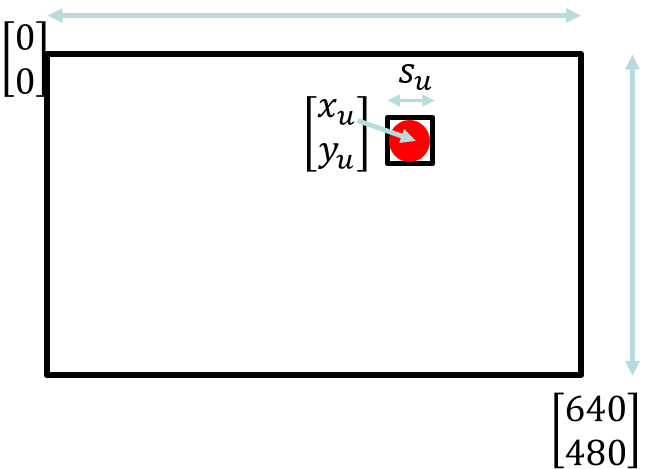
\includegraphics[width=0.5\textwidth]{computerVision}
	\end{center}
	\caption{Computer vision tracking model}
	\label{fig:computervis}
\end{figure}

\medskip

The midpoint of the target in the ideal undistorted image is $\pu = \mat{ x_u & y_u }^{T}$. The center of the undistorted image is $c_x$ in the x direction and $c_y$ in the y direction. The focal lengths in the x and y directions are $f_x$ and $f_y$, respectively. These parameters are found through the camera calibration routine, explained in detail below. The measurements of the center of the target and its width are related to the hidden state $\pspr = \mat{ x_s & y_s & z_s }^{T}$ in the following way: 

\[
    \y = h(\x)
        = \mat{x_u \\ y_u \\ s_{u} }
        = \mat{ \frac{f_x x_s}{z_s} + c_x \\ 
             \frac{f_y y_s}{z_s} + c_y \\ 
             \frac{s_c}{z_s \sqrt{\frac{1}{f_x^{2}} + \frac{1}{f_y^{2}}}}
           }
\]

These relationships are found through using a simple pin-hole camera model \cite{Tsai1987}.


\subsubsection{Camera Calibration}

The measurement model requires knowledge of the intrinsic camera parameters, $f_x, f_y, c_x, c_y$, and the radial and tangential distortion factors. There are two steps to translating a point from camera coordinates to image coordinates \cite{Tsai1987}. First, the pin-hole camera model shows how to find the ideal image coordinates of an object, $(\mathbf{x_u}, \mathbf{y_u})$ based on the position of the object in camera coordinates, $\pspr = (x, y, z)$: 

$$ \mathbf{x_u} = f_x \frac{x}{z} $$
$$ \mathbf{y_u} = f_y \frac{y}{z} $$

Second, the radial and tangential distortion relations show how the actual image coordinates, $(\mathbf{x_u}, \mathbf{y_u})$, relate to the image coordinates on the actual or distorted image plane, $(\mathbf{x_d}, \mathbf{y_d})$. The radial distortion correction equation is as follows: \\

$$ \mathbf{x_u} = x_d (1 + k_1 r^2 + k_2 r^4 + k_3 r^6) $$
$$ \mathbf{y_u} = y_d (1 + k_1 r^2 + k_2 r^4 + k_3 r^6) $$

and the tangential distortion equation is given by, 

$$ \mathbf{x_u} = x_d + (2 p_1 x y + p_2 (r^2 + 2x^2))$$
$$ \mathbf{y_u} = y_d + (p_1 (r^2 + 2y^2) + 2p_2 x y)$$

Thus, the five distortion parameters are summarized in a vector $D$: 

$$D = \mat{ k_1 & k_2 & p_1 p_2 & k_3 }$$

The calibration parameters are discovered by using an open source implementation provided by OpenCV. The camera collects a series of images that contain a checkerboard pattern. The calibration computes the transformation from the image coordinates of the checkerboard to its real world coordinates. The calibration images look like the ones in figure 1 below. 

\begin{figure}[H]
    \begin{center}$
        \begin{array}{cc}
            \includegraphics[width=0.2\textwidth]{image1} &
            \includegraphics[width=0.2\textwidth]{image2} \\
            \includegraphics[width=0.2\textwidth]{image3} &
            \includegraphics[width=0.2\textwidth]{image4} \\
        \end{array}$
    \end{center}
    \caption{Camera calibration routine}
    \label{fig:cameracalib}
\end{figure}

\subsubsection{Object Tracking}

The signal processing layer contains an object tracker to find the rear of the interaction tool in each frame. Since a robust estimate of the object size in each image is required, its edges must be estimated as exactly as possible. One simple way to estimate the edges of the spherical tracking target is to segment the tracking target from the background by using color. The color of the object is used determine which pixels belong to it and which to not. Additionally, the color-based object tracking must happen in real time. To meet the demands of real-time, color-based object tracking, the CamShift algorithm was chosen \cite{bradski1998}.

%%%%%%%%%%%%%%%%%%%%%%%%%%%%%%%%%%%%%%%%%%%%%%%%%%%%%%%%%%%%%%%%%%%%%%%%%%%%%%%
%% Dynamic measurement model

\subsection{Dynamic Measurement Model}

Since the user's movement of the interaction tool is voluntary, no assumptions can be made about its overall trajectory. However, human-motion objeys minimum-jerk constraints \cite{flash1985}. Since the jerk of the tool's motion is small, it can be modelled as a white-noise process. The dynamical model for the tool's motion along the $x$ axis is estimated by the discrete time state-space model

$$ \vec{x}_{k+1} = \mat{1 & \Delta t \\ 0 & 1} \mat{x \\ \xd} + \mat{0 \\ \Delta t} \xdd  + \mat{0 \\ 1} w_k $$

where $w_k$ is the jerk. Additionally, the motion of the tool is assumed to be coordinate uncoupled, since the user is free to move the tool in any direction. Therefore this same model can be extended to motion along the $y$ and $z$ axes as well.


%%%%%%%%%%%%%%%%%%%%%%%%%%%%%%%%%%%%%%%%%%%%%%%%%%%%%%%%%%%%%%%%%%%%%%%%%%%%%%%
%% Performance Analysis
%%%%%%%%%%%%%%%%%%%%%%%%%%%%%%%%%%%%%%%%%%%%%%%%%%%%%%%%%%%%%%%%%%%%%%%%%%%%%%%
\section{Performance Analysis}

\subsection{Estimation Error}

Given the tool model $ \pfe = \pre + \ple $, the overall error covariance $\Ppf$ is a function of the error due to the position estimation and the error to the orientation estimation. Since the estimation of $\pr$ and $\pl$ occur independently, it is reasonable to assume that the errors in the estimation of these vectors is not correlated. Thus, the covariances of the errors for these two vectors simply add to yield the covariance of the error for the tool front: 

\begin{equation} \label{eq:Ppf}
    \Ppf =  \Ppr + \Ppl
\end{equation}

\subsection{Covariance Transformations}

Here are three properties of covariance transformations, useful for analysing the performance of the tracking system as a whole: 

\medskip

(1) Given two independent random variables $X$, $Y$, and their sum $Z = X + Y$ how does the covariance of $Z$ $\Sigma_Z$ relate to the covariances $\Sigma_X$ and $\Sigma_Y$ of $X$ and $Y$, respectively? In this case the covariances simply sum so that 

$$ \Sigma_Z = \Sigma_X + \Sigma_Y $$

\medskip

(2) Given two random variables $X$ and $Y$ related by the linear operator $T$ so that $ Y = T X $ how does the covariance of $Y$ relate to the covariance of $X$?  If $\Sigma_X$ is the covariance of $X$ and $\Sigma_Y$ is the covariance of $Y$, then 

$$ \Sigma_Y = T \Sigma_X T^T $$  

\medskip

(3) Given two random variables $X$ and $Y$, and the non-linear relationship that $Y = f(X)$, how does the covariance of $Y$ change with the covariance of $X$? As a first-order approximation, the randomness of $Y$ can be approximated as a linear function of $X$ \cite{haralick1996}: 

\begin{equation} \label{eq:firstorderdev}
    Y - \mu_Y = T (X - \mu_X)
\end{equation}

Now, given the linear relationship, $Y - \mu_Y = T (X - \mu_X) $, the covariance of $Y$ is related to the covariance of $X$ by 

$$ \Sigma_Y = T \Sigma_X T^{T} $$

using property (2) of the covariance transformation under a linear operator.

\subsection{Estimation Error for $\ple$: Finding position error due to orientation error}

How do errors in the orientation estimation lead to errors the tool position estimation? In the tool model, the position of the front of the tool is estimated from three pieces of information: the position of the rear of the tool $\pr$, the orientation of the tool $\At$, and the tool length in body coordinates $\plpr$. This relationship is described by the equation 

$$ \pf = \pr + \pl = \pr + \At^{T} \plpr $$ 

There is no error in the measurement of $\plpr$; that is a well known parameter of the interaction tool. The error in $\pl$ comes from the estimation of the rotation matrix from body coordinates to world coordinates. 

\medskip

The attitude matrix $\At$ is parameterized by the quaternion $\qt$ estimated from the EKF so that $\pl = \At(\qt)^{T} \plpr$. This expression is helpful because it describes the tool span vector $\pl$ as a function of $\qt$. The relationship between $\pl$ and $\qt$ must be linearlized in order to understand how errors in the estimation of $\qt$ translate to errors in $\pl$. 

\medskip

Let the small deviations in the orientaiton be represented by the error quaternion $\dq$ so that $\pl = \A(\dq) \At(\qt)^{T} \plpr$, where $\A(\dq)$ is the attitude matrix parameterized by the orientation error. Then, the goal here is to linearize the relationship between $\pl$ and $\dq$, and to accomplish we find the matrix first-order derivative of $\pl$ with respect to the three dimensional representation of the error quaternion $\dqvec$: 

$$ \deldq = \ddq \A(\dq) \At(\qt)^T \plpr $$

Now simplify $\A(\dq)$ using the assumptions that $\dqw \approx 1$ and $|\dqvec| \approx 0$, both of which will be true for small errors:

$$ \A(\dq) = (|\dqw|^2 - |\dqvec|) I_{3x3} + 2 \dqvec \dqvec^T - 2\dqw\crossmat{\dqvec}  = I_{3x3} - 2\crossmat{\dqvec} $$

Pplugging in this expression for $\A(\dq)$: 

$$ \deldq = \ddq (I_{3x3} - 2\crossmat{\dqvec}) \At(\qt)^T \plpr $$

Note that $\At(\qt)^T \plpr$ is a constant vector -- in fact it is simply the estimate for $\pl$! 

$$ \deldq = \ddq( I_{3x3} \pl - 2 \crossmat{\dqvec} \pl )  = -2 \ddq \crossmat{\dqvec} \pl $$

The quantity $\crossmat{\dqvec} \pl$ is simply $\dqvec \times \pl = -\pl \times \dqvec$. Therefore, 

$$ \deldq = -2 \ddq (-\pl \times \dqvec) = 2 \crossmat{\pl} \ddq \dqvec = 2 \crossmat{\pl} $$

Now we can write deviations in $\pl$ as a linear function of the quaternion error or angular error ( $\dqvec = \frac{1}{2} \dtvec$ ): 

$$ \delta\pl = 2 \crossmat{ \At(\qt)^T \plpr } \dqvec  =  \crossmat{ \At(\qt)^T \plpr } \dtvec $$

This is written in the form of Equation \ref{eq:firstorderdev}. Thus, if $\Ptt$ is the covariance of the estimation of the tool's orientation, then the covariance $\Ppl$ of $\pl$ is

\begin{equation} \label{eq:plcovariance}
    \Ppl = \crossmat{ \At(\qt)^T \plpr } \Ptt \crossmat{ \At(\qt)^T \plpr }^T 
        = \At(\qt)^T \crossmat{\plpr} \Ptt \crossmat{\plpr}^T \At(\qt)
\end{equation}


% Covariance equations
% $$ \Pprpr = \Ppspr + \crossmat{\pspr} \Pacpr \crossmat{\pspr}^T $$
% $$ \Ppr = \Acinv ( \Ppspr + \crossmat{\pspr} \Pacpr \crossmat{\pspr}^T ) (\Acinv)^T + \Ppc $$
% $$ \Ppf = \Ppr + \Atinv \crossmat{\pl} \Patpr \crossmat{\pl}^T (\Atinv)^T $$
% $$ \Ppfpr = \Ad ( \Ppf + \Ppd ) \Ad{^T} $$
% $$ \Ppfpr = \Ppspr + \crossmat{\pspr} \Pacpr \crossmat{\pspr}^T + \Atpr \crossmat{\pl} \Patpr \crossmat{\pl}^T (\Atpr)^T + 2\Ad\Ppd\Ad{^T} $$

%%%%%%%%%%%%%%%%%%%%%%%%%%%%%%%%%%%%%%%%%%%%%%%%%%%%%%%%%%%%%%%%%%%%%%%%%%%%%%%
%% Conclusion
%%%%%%%%%%%%%%%%%%%%%%%%%%%%%%%%%%%%%%%%%%%%%%%%%%%%%%%%%%%%%%%%%%%%%%%%%%%%%%%
\section{Conclusion}

%%%%%%%%%%%%%%%%%%%%%%%%%%%%%%%%%%%%%%%%%%%%%%%%%%%%%%%%%%%%%%%%%%%%%%%%%%%%%%%
%% Future Work
%%%%%%%%%%%%%%%%%%%%%%%%%%%%%%%%%%%%%%%%%%%%%%%%%%%%%%%%%%%%%%%%%%%%%%%%%%%%%%%
\section{Future Work}


\bibliographystyle{ieeetr}
\bibliography{references}

\end{flushleft}
% \end{multicols}
\end{document} 
